\documentclass[12pt]{article}

% ── Packages ──────────────────────────────────────────────
\usepackage[margin=1in]{geometry}
\usepackage{xeCJK}
\setCJKmainfont{AR PL UMing TW}
\usepackage{graphicx}
\usepackage{booktabs}
\usepackage{hyperref}
\usepackage{amsmath}
\usepackage{float}
\usepackage{enumitem}
\usepackage{caption}
\usepackage{subcaption}
\usepackage{natbib}
\usepackage{setspace}
\usepackage{minted}
\usepackage{xcolor}
\usepackage{tabularx}

\setstretch{1.0}
\setlength{\parskip}{4pt}
\setlength{\parindent}{0pt}
\captionsetup{font=small}

\setminted{
  fontsize=\scriptsize,
  breaklines=true,
  numbers=left,
  numbersep=5pt,
  frame=single,
  framesep=2mm,
}

\title{\Large\textbf{Sentiment Classification of Taiwanese Restaurant Reviews\\from Google Maps}\\[6pt]
\large AI Capstone Project \#1 --- NYCU Spring 2026}
\author{Student ID: 313553058}
\date{}

% ══════════════════════════════════════════════════════════
\begin{document}
\maketitle

\textbf{GitHub Repository:} \url{https://github.com/PLACEHOLDER/ai-capstone-project1}
\hfill \textit{(to be updated before submission)}

% ══════════════════════════════════════════════════════════
\section{Research Question and Motivation}

Can we automatically classify the sentiment of Taiwanese restaurant reviews from Google Maps into positive, neutral, and negative categories using traditional ML and transfer learning approaches?

Online restaurant reviews heavily influence dining decisions in Taiwan.
Google Maps is one of the most popular platforms, with reviews written predominantly in Traditional Chinese.
However, star ratings alone can be misleading---a 3-star review in Taiwanese consumer culture often signals dissatisfaction rather than true neutrality.
This project aims to (1)~construct a novel dataset of Taiwanese food reviews via web crawling, (2)~compare traditional NLP pipelines (TF-IDF + SVM/LR) with BERT-based transfer learning, and (3)~investigate how the ambiguous 3-star class affects classification performance.

We also demonstrate a practical application: a tool that analyzes any restaurant's Google Maps reviews to produce sentiment trend reports, which could help restaurant owners identify service or quality issues over time.

% ══════════════════════════════════════════════════════════
\section{Dataset Documentation}

\subsection{Data Type and Source}

The dataset consists of text reviews crawled from \textbf{Google Maps} using Playwright~\citep{playwright} with a headless Chromium browser.
Each sample contains: \texttt{review\_text} (Traditional Chinese), \texttt{rating} (1--5 stars), \texttt{restaurant} name, \texttt{area} (city/region), \texttt{date} (relative), and \texttt{likes} count.
Labels are derived from star ratings: 1--2$\star$ = negative (0), 3$\star$ = neutral (1), 4--5$\star$ = positive (2).

\subsection{Amount and Composition}

\begin{table}[H]
\centering
\caption{Dataset overview.}
\label{tab:dataset}
\begin{tabular}{lr}
\toprule
\textbf{Attribute} & \textbf{Value} \\
\midrule
Raw reviews collected & 6{,}547 \\
After cleaning & 6{,}509 \\
Unique restaurants & 218 \\
Regions covered & 18 \\
Positive (4--5$\star$) & 5{,}162 (79.3\%) \\
Neutral (3$\star$) & 664 (10.2\%) \\
Negative (1--2$\star$) & 683 (10.5\%) \\
Avg.\ review length & 106.2 chars \\
Median review length & 72 chars \\
Mean star rating & 4.18 \\
\bottomrule
\end{tabular}
\end{table}

The dataset exhibits severe class imbalance: positive reviews dominate at 79.3\%, while neutral and negative classes each constitute roughly 10\%.
This imbalance is inherent to online review platforms---most diners leave reviews only when satisfied.

\begin{figure}[H]
\centering
\begin{subfigure}[b]{0.48\textwidth}
  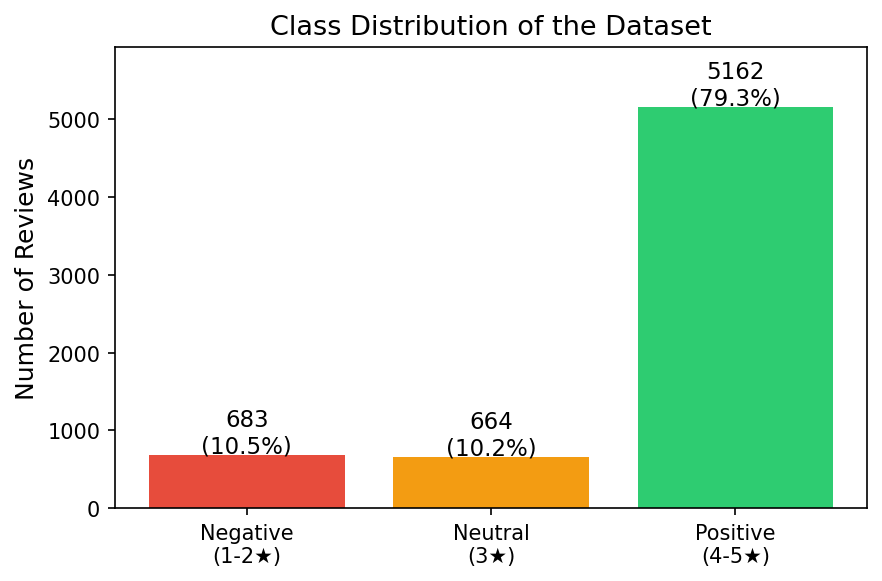
\includegraphics[width=\textwidth]{figures/eda_class_distribution.png}
  \caption{Class distribution.}
\end{subfigure}
\hfill
\begin{subfigure}[b]{0.48\textwidth}
  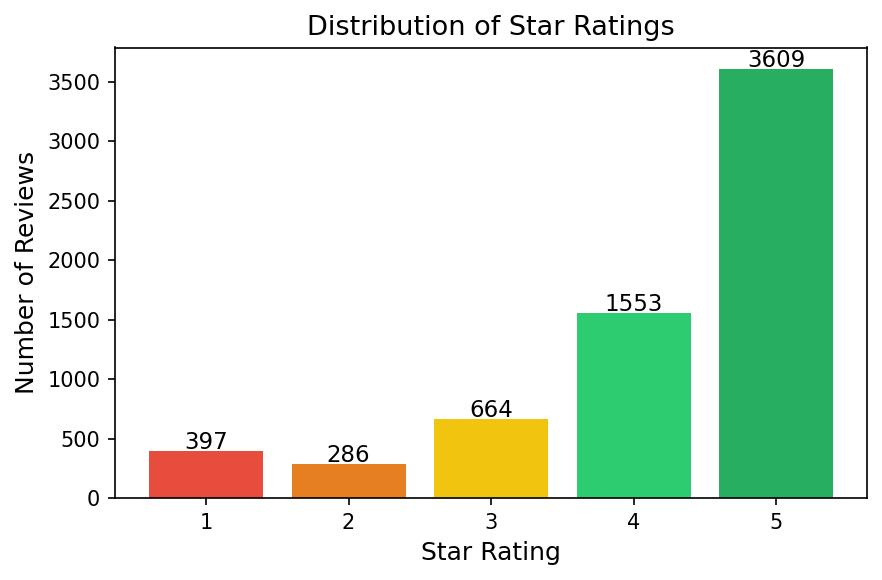
\includegraphics[width=\textwidth]{figures/eda_rating_distribution.png}
  \caption{Star rating distribution.}
\end{subfigure}
\caption{Dataset composition. 5-star reviews dominate, creating severe class imbalance.}
\label{fig:eda}
\end{figure}

\subsection{Data Collection Process}

We constructed 45 search queries spanning 10 cities (Taipei, New Taipei, Taichung, Tainan, Kaohsiung, Hsinchu, Chiayi, Keelung, Yilan, Hualien) and 8 night markets across Taiwan.
For each query, the crawler: (1)~searches on Google Maps, (2)~iterates through restaurant results, (3)~clicks the reviews tab, (4)~scrolls to load all reviews, (5)~expands truncated text, and (6)~extracts structured data.

Anti-blocking measures include: random delays (2--5s between actions), restaurant rotation every 5 entries, randomized query order, and a realistic user-agent string.

\subsection{Data Cleaning}

Cleaning removed 38 reviews (99.4\% retention): empty/NaN text, reviews shorter than 5 characters, reviews without Chinese characters, exact duplicates, and entries with rating = 0 (extraction failures).

\subsection{Examples}

\begin{table}[H]
\centering
\caption{Sample reviews from the dataset.}
\label{tab:examples}
\small
\begin{tabularx}{\textwidth}{c c X}
\toprule
\textbf{Rating} & \textbf{Label} & \textbf{Review Text (translated summary)} \\
\midrule
5$\star$ & Positive & ``Delicious braised pork rice, generous portions, friendly boss. Will visit again!'' \\
3$\star$ & Neutral & ``Food is okay, but the environment could be cleaner. Prices are average.'' \\
1$\star$ & Negative & ``Extremely rude staff, dirty dishes with leftover food, meat overcooked and too salty.'' \\
\bottomrule
\end{tabularx}
\end{table}

% ══════════════════════════════════════════════════════════
\section{Methods}

Our approach evolves through three stages, from a traditional NLP baseline to BERT-based transfer learning.

\subsection{Stage 1: TF-IDF + Classical ML}

\textbf{Tokenization.}
Chinese text requires word segmentation.
We use jieba~\citep{jieba} in precise mode with a custom dictionary containing domain-specific terms (e.g., ``CP值'' [value for money], ``踩雷'' [bad experience], ``排隊'' [queuing]).
Stopwords are filtered using a curated Chinese stopword list, and tokens with length $\leq 1$ are removed.

\textbf{Feature extraction.}
We apply TF-IDF vectorization (\texttt{max\_features}=5{,}000) followed by TruncatedSVD~\citep{halko2011svd} for dimensionality reduction to 150 dimensions, which retains 25.2\% of the total variance.

\textbf{Classifiers.}
We train two models: (1)~Logistic Regression (LR) with L2 regularization (\texttt{max\_iter}=1000), and (2)~SVM with RBF kernel (\texttt{C}=1.0, $\gamma$=\texttt{scale}).
Both support sample weighting via $w_i = 1 + \log(1 + \text{likes}_i)$ to give more influence to highly-liked reviews.

\subsection{Stage 2: BERT Embeddings + Classical ML}

To capture deeper semantic features, we use XLM-RoBERTa-large~\citep{conneau2020xlmr} fine-tuned on XNLI~\citep{conneau2018xnli} (\texttt{joeddav/xlm-roberta-large-xnli}) as a \textit{feature extractor}.
We perform mean pooling over the last hidden states to obtain 1{,}024-dimensional embeddings for each review.
These embeddings replace TF-IDF+SVD features while keeping our trained LR/SVM classifiers---this constitutes \textbf{transfer learning}, where BERT provides the representation and our classifiers are the learned components.

We also run BERT in a \textbf{zero-shot} configuration as a baseline, classifying reviews into ``positive,'' ``neutral,'' and ``negative'' without any training on our data.

\subsection{Stage 3: Binary Classification (3-Star as Negative)}

Based on our experiment (Section~\ref{sec:neutral}), we reclassify 3-star reviews as negative, reducing the task to binary (satisfied vs.\ dissatisfied).
This reflects a cultural insight: in Taiwan, giving 3 out of 5 stars typically signals dissatisfaction rather than neutrality.

\subsection{Evaluation}

All models are evaluated using \textbf{5-fold Stratified Cross-Validation}~\citep{scikit-learn}.
Metrics include: Accuracy, Macro F1, Macro Precision, Macro Recall, and AUROC (One-vs-Rest).
We use Macro F1 as the primary metric since it accounts for class imbalance.

% ══════════════════════════════════════════════════════════
\section{Experiments and Results}

\subsection{Baseline Model Comparison}

\begin{table}[H]
\centering
\caption{Model comparison (5-fold CV, 3-class). Best values in bold.}
\label{tab:models}
\begin{tabular}{lcccc}
\toprule
\textbf{Model} & \textbf{Accuracy} & \textbf{F1 Macro} & \textbf{Precision} & \textbf{Recall} \\
\midrule
TF-IDF + LR      & 0.818 & 0.449 & 0.703 & 0.415 \\
TF-IDF + SVM     & 0.822 & 0.457 & 0.509 & 0.448 \\
BERT zero-shot   & 0.815 & 0.559 & ---   & ---   \\
BERT + SVM       & 0.798 & 0.328 & 0.599 & 0.350 \\
\textbf{BERT + LR} & \textbf{0.842} & \textbf{0.636} & \textbf{0.652} & \textbf{0.625} \\
\bottomrule
\end{tabular}
\end{table}

All models achieve $\sim$82\% accuracy, largely because predicting ``positive'' for everything already yields 79.3\%.
The key differentiator is Macro F1: \textbf{BERT+LR outperforms all others at 0.636}, surpassing even the zero-shot baseline (0.559).
Notably, BERT+SVM performs worst (F1=0.328)---the RBF kernel struggles in the 1{,}024-dimensional BERT space.

\begin{figure}[H]
\centering
\begin{subfigure}[b]{0.48\textwidth}
  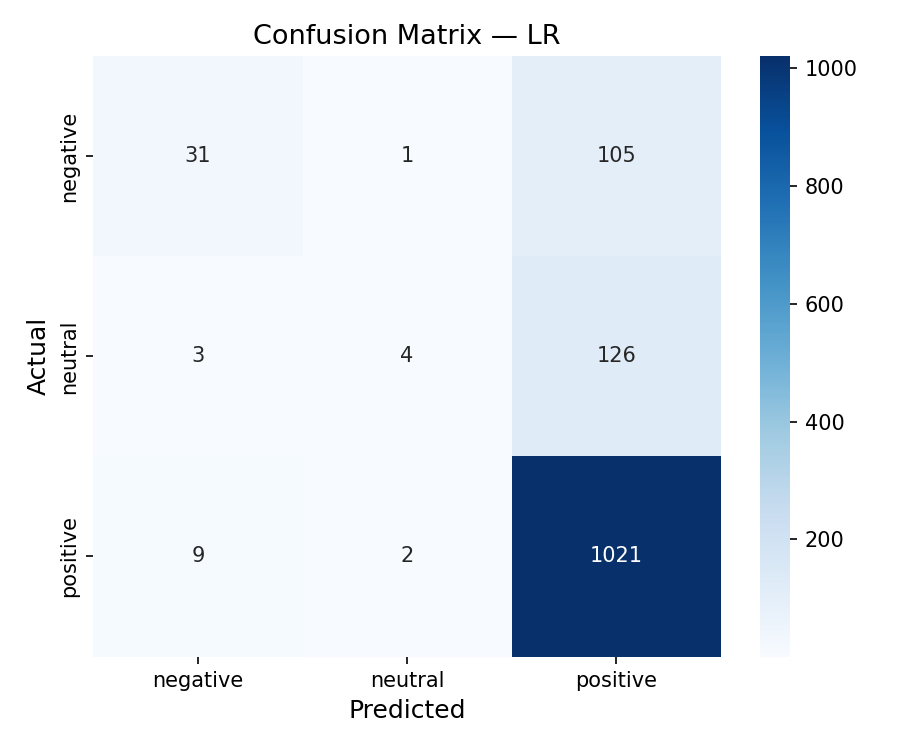
\includegraphics[width=\textwidth]{figures/confusion_matrix_LR.png}
  \caption{TF-IDF + LR}
\end{subfigure}
\hfill
\begin{subfigure}[b]{0.48\textwidth}
  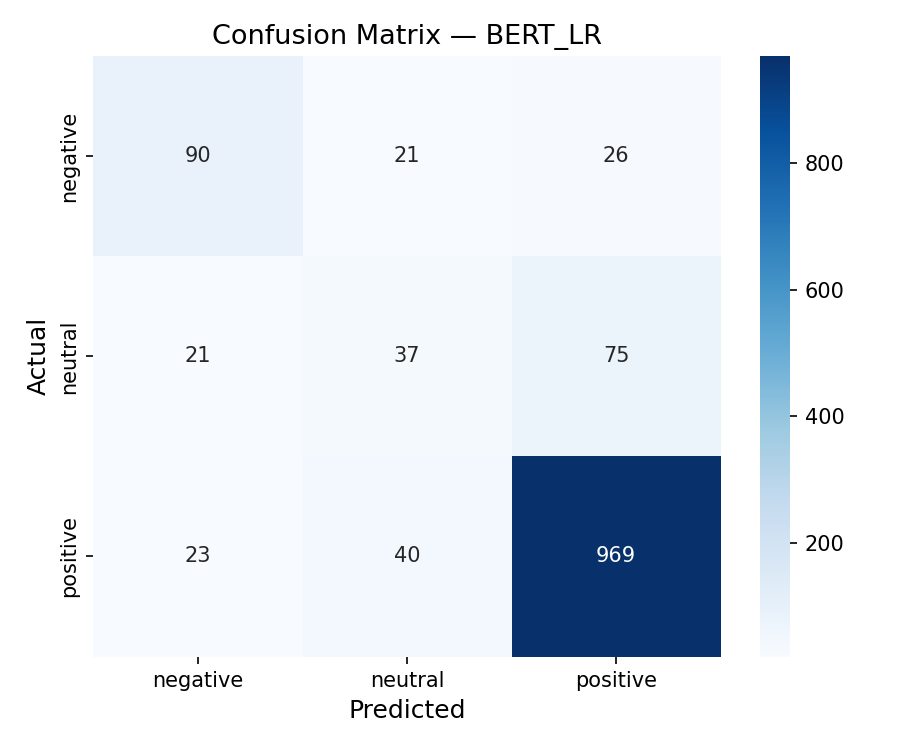
\includegraphics[width=\textwidth]{figures/confusion_matrix_BERT_LR.png}
  \caption{BERT + LR}
\end{subfigure}
\caption{Confusion matrices. BERT+LR significantly improves neutral/negative recall.}
\label{fig:cm}
\end{figure}

\subsection{Experiment 1: Learning Curve}

We train LR with 10\%, 25\%, 50\%, 75\%, and 100\% of the data to study how performance scales.

\begin{table}[H]
\centering
\caption{Learning curve --- Logistic Regression (5-fold CV).}
\label{tab:learning}
\begin{tabular}{rcccc}
\toprule
\textbf{Train Size} & \textbf{Train F1} & $\pm$ & \textbf{Val F1} & $\pm$ \\
\midrule
520  (10\%) & 0.299 & 0.006 & 0.295 & 0.000 \\
1301 (25\%) & 0.343 & 0.015 & 0.323 & 0.016 \\
2603 (50\%) & 0.422 & 0.012 & 0.388 & 0.023 \\
3905 (75\%) & 0.452 & 0.009 & 0.422 & 0.024 \\
5207 (100\%) & 0.466 & 0.008 & 0.449 & 0.022 \\
\bottomrule
\end{tabular}
\end{table}

Performance improves steadily with more data, and the gap between training and validation F1 is small, suggesting the model is not overfitting.
The curve has not plateaued at 100\%, indicating that collecting more data would likely continue to improve results.

\subsection{Experiment 2: Class Balance}

We compare three strategies to address the 79:10:10 class imbalance.

\begin{table}[H]
\centering
\caption{Class balance strategies --- LR (5-fold CV).}
\label{tab:balance}
\begin{tabular}{lcccc}
\toprule
\textbf{Strategy} & \textbf{Accuracy} & \textbf{F1 Macro} & \textbf{Precision} & \textbf{Recall} \\
\midrule
Original           & 0.811 & 0.432 & 0.703 & 0.415 \\
Balanced weights   & 0.647 & \textbf{0.516} & 0.506 & \textbf{0.597} \\
SMOTE~\citep{chawla2002smote} & 0.656 & 0.506 & 0.495 & 0.577 \\
\bottomrule
\end{tabular}
\end{table}

Using \texttt{class\_weight='balanced'} sacrifices 16 points of accuracy but gains 19.5\% in F1 Macro.
SMOTE produces similar results.
The accuracy drop is expected: the model now correctly classifies more minority samples at the cost of some majority-class errors.

\subsection{Experiment 3: Dimensionality Reduction (TruncatedSVD)}

\begin{table}[H]
\centering
\caption{Effect of SVD dimensionality --- LR (5-fold CV).}
\label{tab:svd}
\begin{tabular}{lccc}
\toprule
\textbf{SVD Dim} & \textbf{Accuracy} & \textbf{F1 Macro} & \textbf{Var.\ Explained} \\
\midrule
None (raw TF-IDF, 5000-d) & \textbf{0.820} & \textbf{0.459} & 100\% \\
50   & 0.811 & 0.416 & 12.1\% \\
100  & 0.817 & 0.443 & 19.4\% \\
150  & 0.818 & 0.449 & 25.2\% \\
200  & 0.818 & 0.454 & 29.9\% \\
\bottomrule
\end{tabular}
\end{table}

Raw TF-IDF slightly outperforms all SVD variants, but the difference is marginal ($<$1\% F1).
Even at 200 dimensions, SVD captures only 30\% of variance, reflecting the extreme sparsity of the TF-IDF matrix.
The 150-d SVD offers a practical trade-off: 97\% of raw TF-IDF performance at 3\% of the dimensionality.

\begin{figure}[H]
\centering
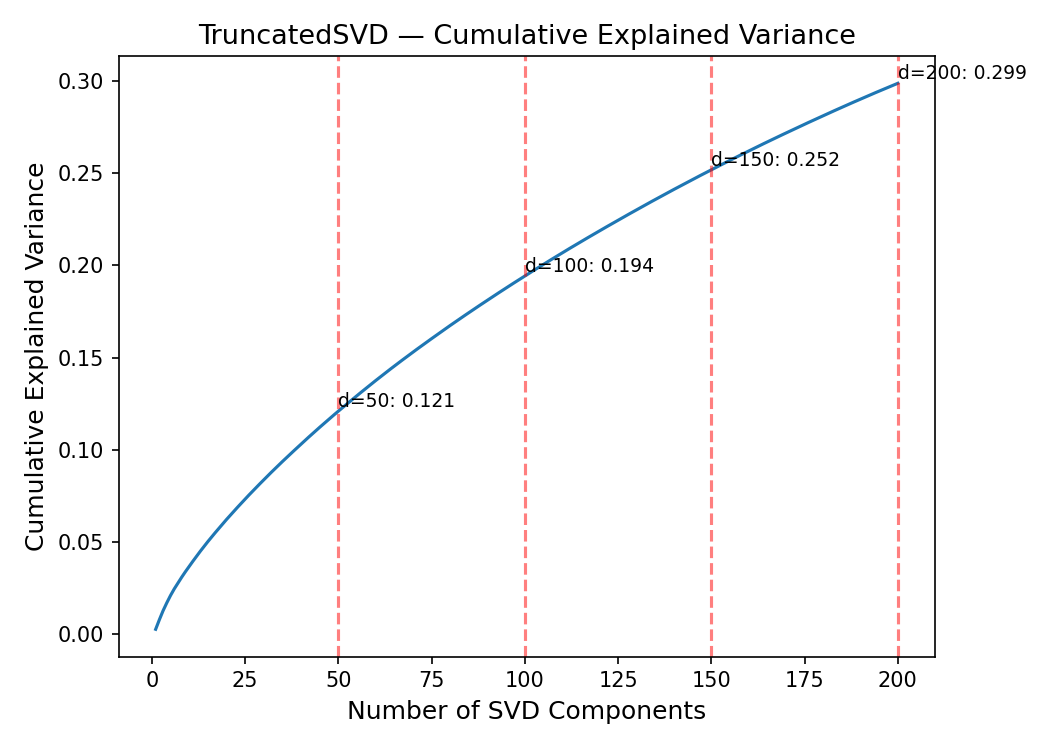
\includegraphics[width=0.55\textwidth]{figures/svd_cumulative_variance.png}
\caption{Cumulative explained variance of TruncatedSVD components.}
\label{fig:svd}
\end{figure}

\subsection{Experiment 4: Neutral Class Handling}
\label{sec:neutral}

The 3-star class is inherently ambiguous.
We test four scenarios to understand its impact.

\begin{table}[H]
\centering
\caption{Effect of neutral class handling --- LR (5-fold CV).}
\label{tab:neutral}
\begin{tabular}{lccccc}
\toprule
\textbf{Scenario} & \textbf{$N$} & \textbf{Classes} & \textbf{Accuracy} & \textbf{F1 Macro} \\
\midrule
3-class (baseline)        & 6{,}509 & 3 & 0.818 & 0.449 \\
Binary (remove neutral)   & 5{,}845 & 2 & 0.898 & 0.595 \\
\textbf{3-star $\to$ negative} & \textbf{6{,}509} & \textbf{2} & \textbf{0.829} & \textbf{0.625} \\
3-star $\to$ positive     & 6{,}509 & 2 & 0.902 & 0.547 \\
\bottomrule
\end{tabular}
\end{table}

\textbf{Reclassifying 3-star as negative yields the best F1 (0.625)}, even better than simply removing neutral samples.
This aligns with a cultural observation: in Taiwan, a 3-star rating on a 5-point scale typically indicates dissatisfaction---consumers who are truly neutral tend not to leave reviews at all.

\subsection{Experiment 5: Data Augmentation}

We apply noise injection (random character deletion/substitution) to augment minority classes.
Results show minimal improvement ($<$1\% F1), consistent with the expectation that character-level noise does not generate semantically meaningful new samples for TF-IDF models.

\subsection{Experiment 6: Feature Representation Comparison}

Combining the best strategies (BERT embeddings + binary classification), we achieve the overall best model.

\begin{table}[H]
\centering
\caption{Best models --- Binary classification with 3-star as negative (5-fold CV).}
\label{tab:best}
\begin{tabular}{lcccc}
\toprule
\textbf{Model} & \textbf{Accuracy} & \textbf{F1 Macro} & \textbf{Precision} & \textbf{Recall} \\
\midrule
TF-IDF + LR (binary) & 0.829 & 0.625 & --- & --- \\
\textbf{BERT + LR (binary)} & \textbf{0.892} & \textbf{0.826} & \textbf{0.846} & \textbf{0.811} \\
BERT + LR (binary, balanced) & 0.849 & 0.792 & 0.771 & 0.826 \\
\bottomrule
\end{tabular}
\end{table}

The final \textbf{BERT+LR binary model achieves F1=0.826}, an 85\% improvement over the TF-IDF baseline.
The progression tells a clear story: better features (BERT) and better label design (binary) are both essential.

% ══════════════════════════════════════════════════════════
\section{Application: Restaurant Analysis Tool (My Friend's Restaurant)}

To demonstrate practical value, we built a tool (\texttt{analyze\_restaurant.py}) that, given a Google Maps URL, automatically: (1)~scrapes all reviews via multi-pass crawling with deduplication, (2)~predicts sentiment using the best model (BERT+LR binary), and (3)~generates monthly trend reports.

\begin{figure}[H]
\centering
\begin{subfigure}[b]{0.58\textwidth}
  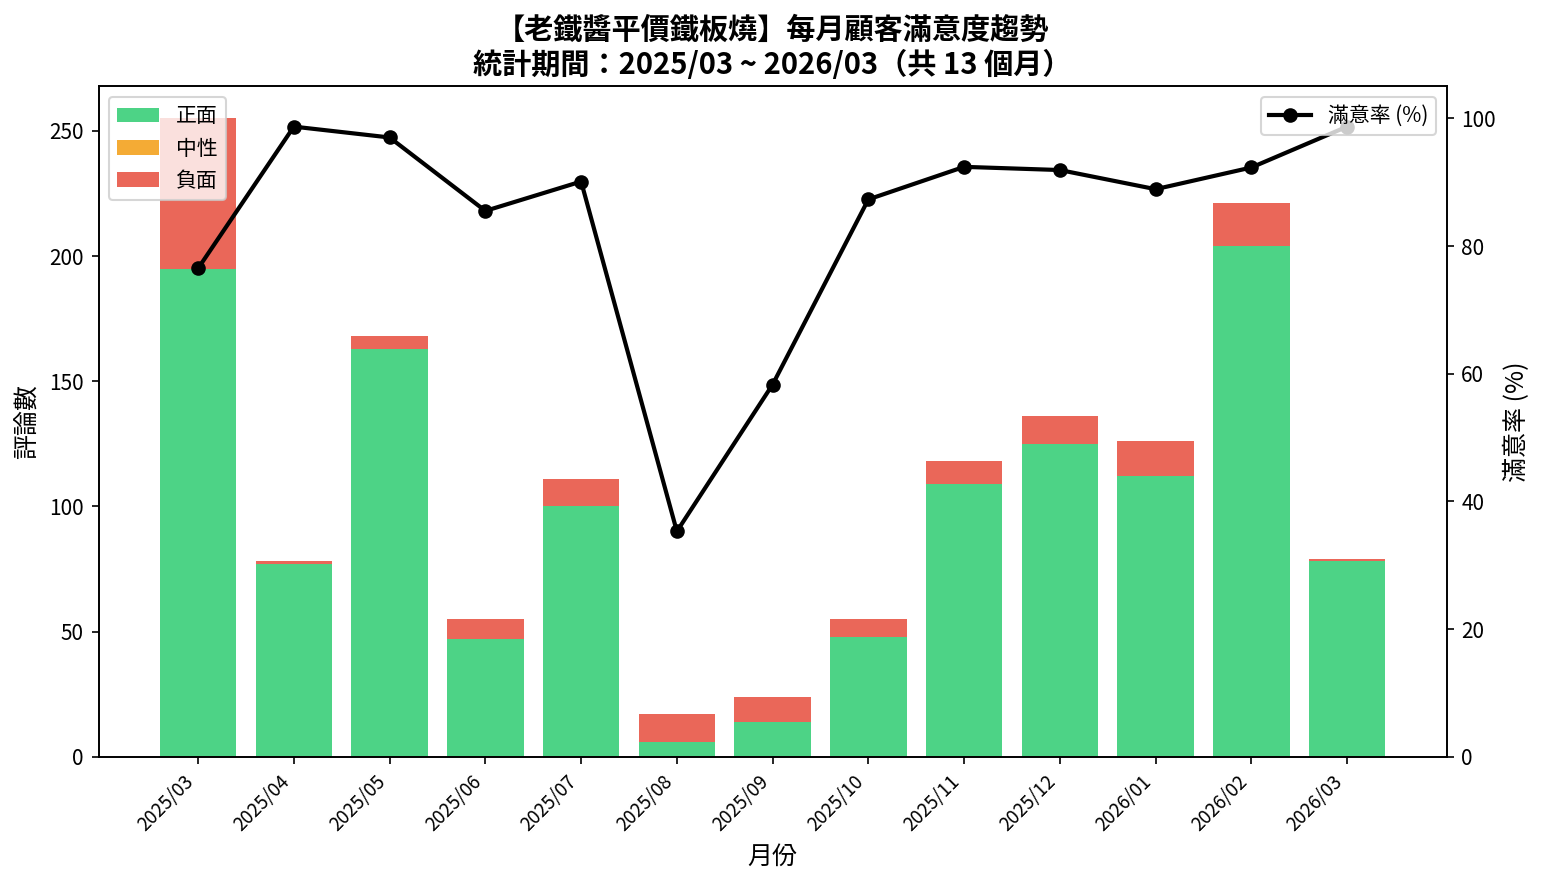
\includegraphics[width=\textwidth]{figures/app_trend.png}
  \caption{Monthly satisfaction trend.}
\end{subfigure}
\hfill
\begin{subfigure}[b]{0.36\textwidth}
  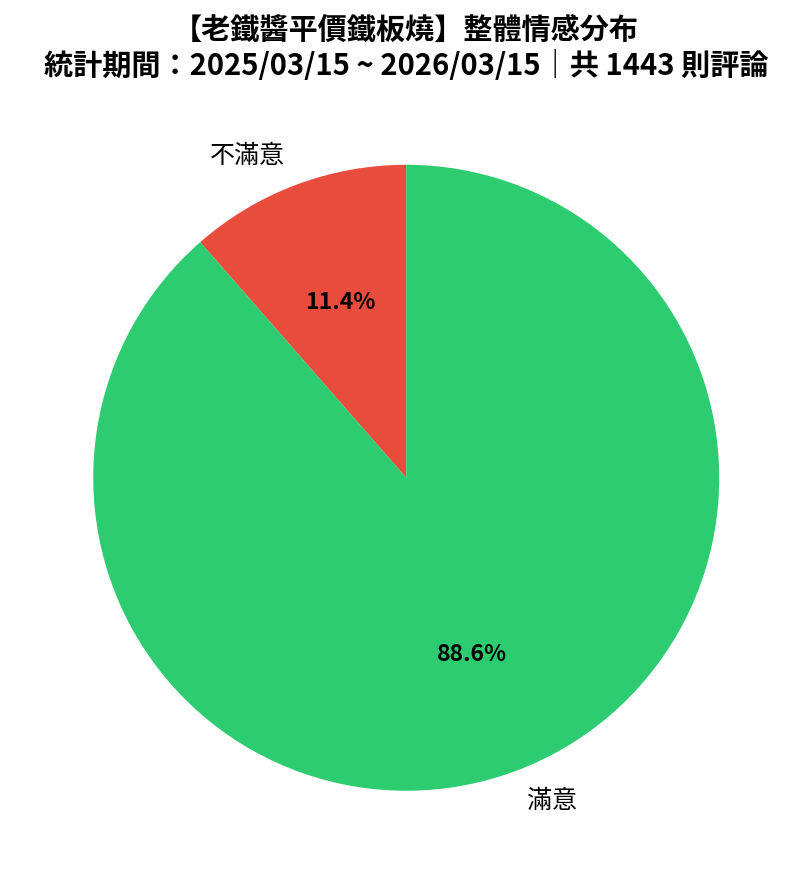
\includegraphics[width=\textwidth]{figures/app_pie.png}
  \caption{Overall sentiment.}
\end{subfigure}
\caption{Application demo on a real restaurant (1{,}443 reviews, 13 months of history).}
\label{fig:app}
\end{figure}

The tool identified a satisfaction dip to 35.3\% in August 2025, which recovered after two months.
Negative review analysis revealed recurring complaints about specific employees and hygiene issues---actionable insights for the restaurant owner.

% ══════════════════════════════════════════════════════════
\section{Discussion}

\textbf{Are the results what we expected?}
Yes and no.
We expected BERT embeddings to outperform TF-IDF (confirmed: +42\% F1), but the magnitude of BERT+SVM's failure (worst overall) was surprising.
The RBF kernel's reliance on Euclidean distance does not suit the high-dimensional, semantically structured BERT space.
Linear models (LR) are a better match.

We also expected 3-class classification to be harder than binary, but the specific finding that ``3-star as negative'' outperforms ``remove neutral'' was a genuinely useful cultural insight.

\textbf{Factors affecting results.}
\begin{enumerate}[nosep]
  \item \textbf{Class imbalance} is the dominant challenge.
    The 79:10:10 ratio means even a naive ``always positive'' classifier reaches 79\% accuracy.
    Macro F1 correctly penalizes this behavior.
  \item \textbf{Review length heterogeneity.}
    Reviews range from 5 to 1{,}000+ characters.
    Short reviews (e.g., ``delicious!'') lack discriminative features for TF-IDF but are captured by BERT's contextual understanding.
  \item \textbf{Sarcasm and mixed sentiment.}
    Some reviews say ``food is great, BUT...'' and then describe serious problems.
    These are hard for all models.
  \item \textbf{Cultural context.}
    Words like ``還好'' (literally ``still okay'') signal negativity in the review context, which TF-IDF cannot capture but BERT can.
\end{enumerate}

\textbf{What would we do with more time?}
\begin{enumerate}[nosep]
  \item Fine-tune BERT on our dataset (currently only used as a frozen feature extractor) to potentially push F1 beyond 0.9.
  \item Implement aspect-based sentiment analysis to separately classify food quality, service, hygiene, and value.
  \item Expand the dataset to 20{,}000+ reviews across more restaurant categories.
  \item Add a temporal component: track how sentiment evolves as restaurants mature.
\end{enumerate}

\textbf{What we learned.}
The most impactful improvements came not from algorithmic tuning but from \textit{understanding the data}: recognizing that 3-star means dissatisfaction in Taiwan, and that BERT embeddings capture cultural nuances that bag-of-words models cannot.
This reinforces the course's emphasis that good models start with good data understanding.

% ══════════════════════════════════════════════════════════
\bibliographystyle{plainnat}
\bibliography{references}

% ══════════════════════════════════════════════════════════
\clearpage
\appendix
\section*{Appendix: Program Code}
\addcontentsline{toc}{section}{Appendix: Program Code}

\subsection*{A.1 Data Collection (\texttt{collect.py}) --- excerpt}
\inputminted[firstline=1,lastline=60]{python}{code/collect.py}

\subsection*{A.2 Preprocessing (\texttt{preprocess.py})}
\inputminted{python}{code/preprocess.py}

\subsection*{A.3 Training (\texttt{train.py})}
\inputminted{python}{code/train.py}

\subsection*{A.4 Evaluation (\texttt{evaluate.py}) --- excerpt}
\inputminted[firstline=1,lastline=80]{python}{code/evaluate.py}

\subsection*{A.5 BERT Feature Extraction (\texttt{bert\_features.py})}
\inputminted{python}{code/bert_features.py}

\subsection*{A.6 BERT+LR Training (\texttt{train\_bert\_svm.py})}
\inputminted{python}{code/train_bert_svm.py}

\subsection*{A.7 Restaurant Analyzer (\texttt{analyze\_restaurant.py}) --- excerpt}
\inputminted[firstline=1,lastline=100]{python}{code/analyze_restaurant.py}

\end{document}
